\documentclass[1p]{elsarticle_modified}
%\bibliographystyle{elsarticle-num}

%\usepackage[colorlinks]{hyperref}
%\usepackage{abbrmath_seonhwa} %\Abb, \Ascr, \Acal ,\Abf, \Afrak
\usepackage{amsfonts}
\usepackage{amssymb}
\usepackage{amsmath}
\usepackage{amsthm}
\usepackage{scalefnt}
\usepackage{amsbsy}
\usepackage{kotex}
\usepackage{caption}
\usepackage{subfig}
\usepackage{color}
\usepackage{graphicx}
\usepackage{xcolor} %% white, black, red, green, blue, cyan, magenta, yellow
\usepackage{float}
\usepackage{setspace}
\usepackage{hyperref}

\usepackage{tikz}
\usetikzlibrary{arrows}

\usepackage{multirow}
\usepackage{array} % fixed length table
\usepackage{hhline}

%%%%%%%%%%%%%%%%%%%%%
\makeatletter
\renewcommand*\env@matrix[1][\arraystretch]{%
	\edef\arraystretch{#1}%
	\hskip -\arraycolsep
	\let\@ifnextchar\new@ifnextchar
	\array{*\c@MaxMatrixCols c}}
\makeatother %https://tex.stackexchange.com/questions/14071/how-can-i-increase-the-line-spacing-in-a-matrix
%%%%%%%%%%%%%%%

\usepackage[normalem]{ulem}

\newcommand{\msout}[1]{\ifmmode\text{\sout{\ensuremath{#1}}}\else\sout{#1}\fi}
%SOURCE: \msout is \stkout macro in https://tex.stackexchange.com/questions/20609/strikeout-in-math-mode

\newcommand{\cancel}[1]{
	\ifmmode
	{\color{red}\msout{#1}}
	\else
	{\color{red}\sout{#1}}
	\fi
}

\newcommand{\add}[1]{
	{\color{blue}\uwave{#1}}
}

\newcommand{\replace}[2]{
	\ifmmode
	{\color{red}\msout{#1}}{\color{blue}\uwave{#2}}
	\else
	{\color{red}\sout{#1}}{\color{blue}\uwave{#2}}
	\fi
}

\newcommand{\Sol}{\mathcal{S}} %segment
\newcommand{\D}{D} %diagram
\newcommand{\A}{\mathcal{A}} %arc


%%%%%%%%%%%%%%%%%%%%%%%%%%%%%5 test

\def\sl{\operatorname{\textup{SL}}(2,\Cbb)}
\def\psl{\operatorname{\textup{PSL}}(2,\Cbb)}
\def\quan{\mkern 1mu \triangleright \mkern 1mu}

\theoremstyle{definition}
\newtheorem{thm}{Theorem}[section]
\newtheorem{prop}[thm]{Proposition}
\newtheorem{lem}[thm]{Lemma}
\newtheorem{ques}[thm]{Question}
\newtheorem{cor}[thm]{Corollary}
\newtheorem{defn}[thm]{Definition}
\newtheorem{exam}[thm]{Example}
\newtheorem{rmk}[thm]{Remark}
\newtheorem{alg}[thm]{Algorithm}

\newcommand{\I}{\sqrt{-1}}
\begin{document}

%\begin{frontmatter}
%
%\title{Boundary parabolic representations of knots up to 8 crossings}
%
%%% Group authors per affiliation:
%\author{Yunhi Cho} 
%\address{Department of Mathematics, University of Seoul, Seoul, Korea}
%\ead{yhcho@uos.ac.kr}
%
%
%\author{Seonhwa Kim} %\fnref{s_kim}}
%\address{Center for Geometry and Physics, Institute for Basic Science, Pohang, 37673, Korea}
%\ead{ryeona17@ibs.re.kr}
%
%\author{Hyuk Kim}
%\address{Department of Mathematical Sciences, Seoul National University, Seoul 08826, Korea}
%\ead{hyukkim@snu.ac.kr}
%
%\author{Seokbeom Yoon}
%\address{Department of Mathematical Sciences, Seoul National University, Seoul, 08826,  Korea}
%\ead{sbyoon15@snu.ac.kr}
%
%\begin{abstract}
%We find all boundary parabolic representation of knots up to 8 crossings.
%
%\end{abstract}
%\begin{keyword}
%    \MSC[2010] 57M25 
%\end{keyword}
%
%\end{frontmatter}

%\linenumbers
%\tableofcontents
%
\newcommand\colored[1]{\textcolor{white}{\rule[-0.35ex]{0.8em}{1.4ex}}\kern-0.8em\color{red} #1}%
%\newcommand\colored[1]{\textcolor{white}{ #1}\kern-2.17ex	\textcolor{white}{ #1}\kern-1.81ex	\textcolor{white}{ #1}\kern-2.15ex\color{red}#1	}

{\Large $\underline{12a_{0092}~(K12a_{0092})}$}

\setlength{\tabcolsep}{10pt}
\renewcommand{\arraystretch}{1.6}
\vspace{1cm}\begin{tabular}{m{100pt}>{\centering\arraybackslash}m{274pt}}
\multirow{5}{120pt}{
	\centering
	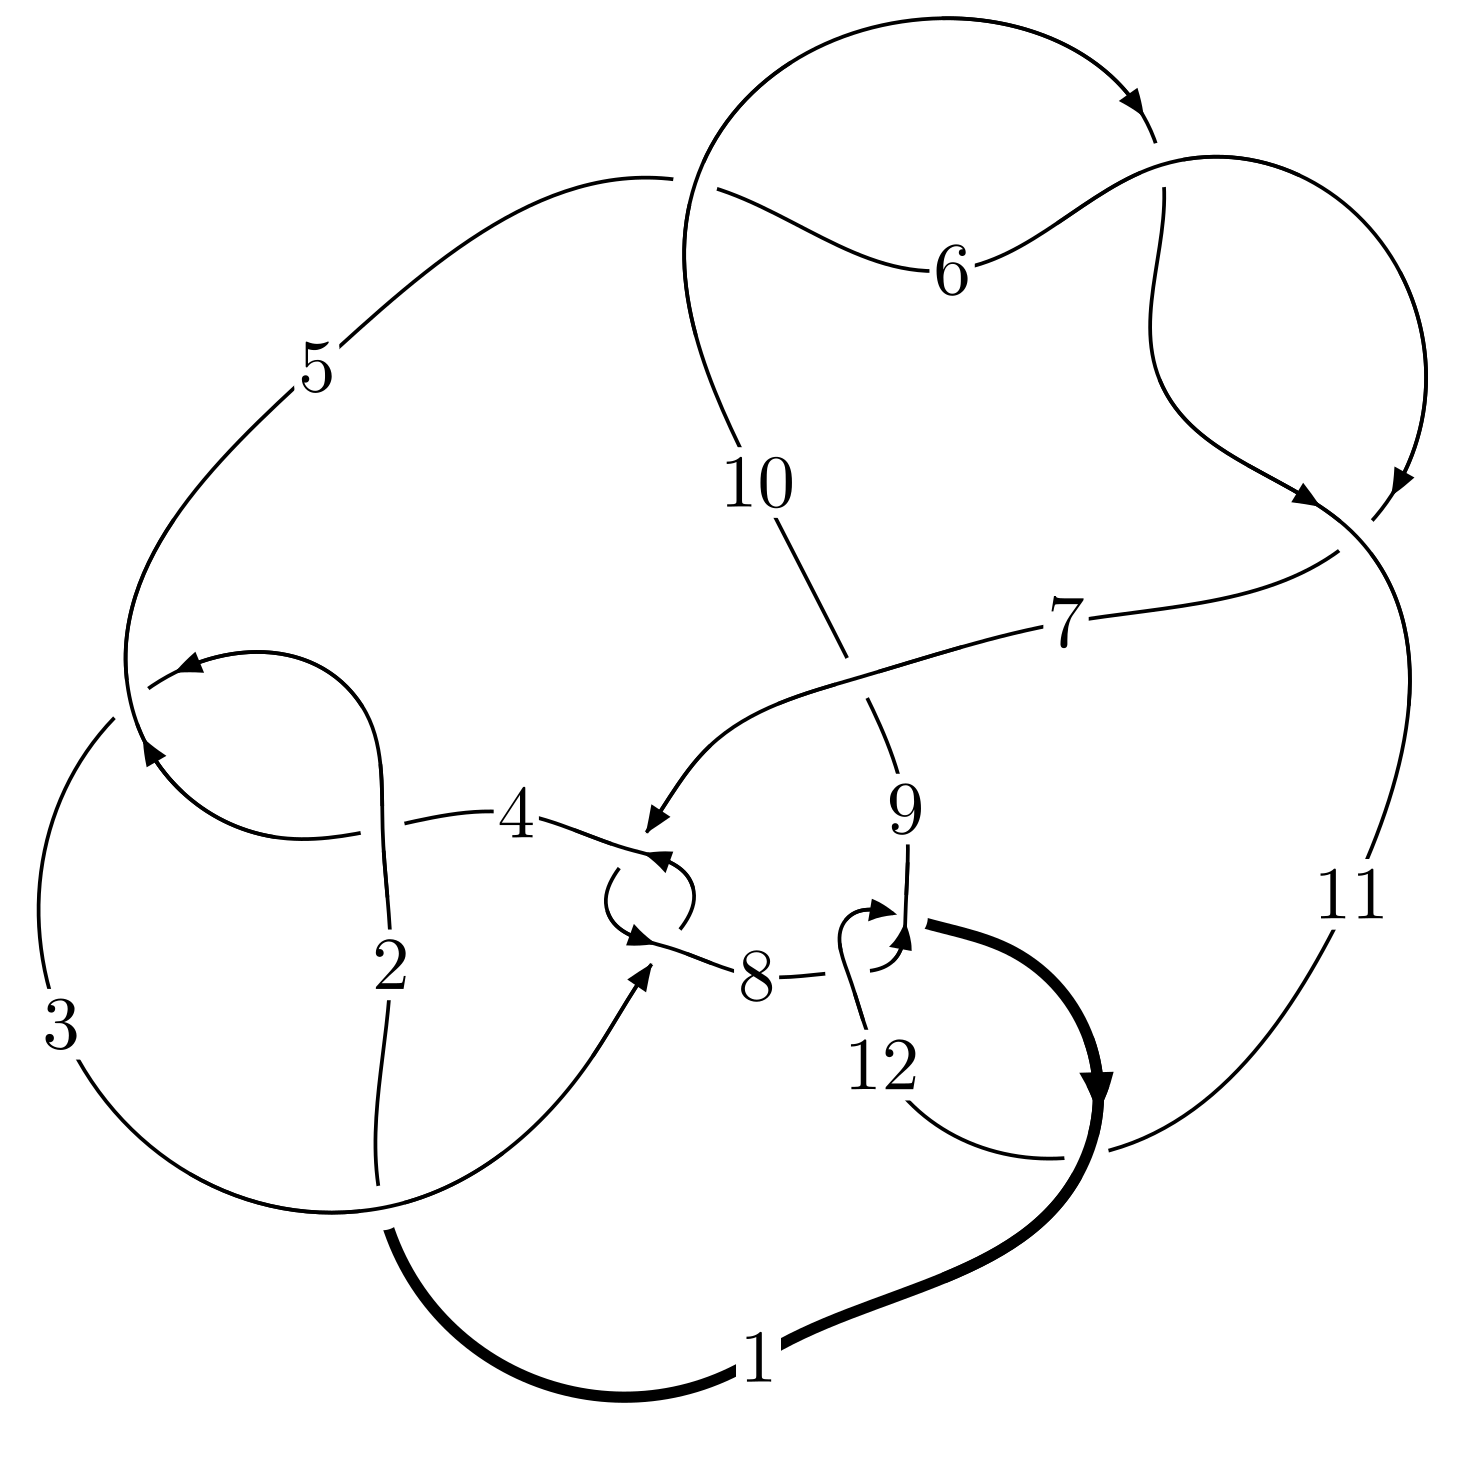
\includegraphics[width=112pt]{../../../GIT/diagram.site/Diagrams/png/893_12a_0092.png}\\
\ \ \ A knot diagram\footnotemark}&
\allowdisplaybreaks
\textbf{Linearized knot diagam} \\
\cline{2-2}
 &
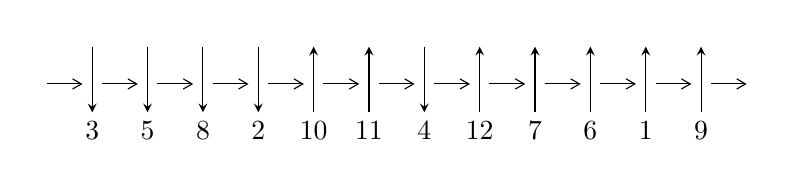
\begin{tikzpicture}[x=20pt, y=17pt]
	% nodes
	\node (C0) at (0, 0) {};
	\node (C1) at (1, 0) {};
	\node (C1U) at (1, +1) {};
	\node (C1D) at (1, -1) {3};

	\node (C2) at (2, 0) {};
	\node (C2U) at (2, +1) {};
	\node (C2D) at (2, -1) {5};

	\node (C3) at (3, 0) {};
	\node (C3U) at (3, +1) {};
	\node (C3D) at (3, -1) {8};

	\node (C4) at (4, 0) {};
	\node (C4U) at (4, +1) {};
	\node (C4D) at (4, -1) {2};

	\node (C5) at (5, 0) {};
	\node (C5U) at (5, +1) {};
	\node (C5D) at (5, -1) {10};

	\node (C6) at (6, 0) {};
	\node (C6U) at (6, +1) {};
	\node (C6D) at (6, -1) {11};

	\node (C7) at (7, 0) {};
	\node (C7U) at (7, +1) {};
	\node (C7D) at (7, -1) {4};

	\node (C8) at (8, 0) {};
	\node (C8U) at (8, +1) {};
	\node (C8D) at (8, -1) {12};

	\node (C9) at (9, 0) {};
	\node (C9U) at (9, +1) {};
	\node (C9D) at (9, -1) {7};

	\node (C10) at (10, 0) {};
	\node (C10U) at (10, +1) {};
	\node (C10D) at (10, -1) {6};

	\node (C11) at (11, 0) {};
	\node (C11U) at (11, +1) {};
	\node (C11D) at (11, -1) {1};

	\node (C12) at (12, 0) {};
	\node (C12U) at (12, +1) {};
	\node (C12D) at (12, -1) {9};
	\node (C13) at (13, 0) {};

	% arrows
	\draw[->,>={angle 60}]
	(C0) edge (C1) (C1) edge (C2) (C2) edge (C3) (C3) edge (C4) (C4) edge (C5) (C5) edge (C6) (C6) edge (C7) (C7) edge (C8) (C8) edge (C9) (C9) edge (C10) (C10) edge (C11) (C11) edge (C12) (C12) edge (C13) ;	\draw[->,>=stealth]
	(C1U) edge (C1D) (C2U) edge (C2D) (C3U) edge (C3D) (C4U) edge (C4D) (C5D) edge (C5U) (C6D) edge (C6U) (C7U) edge (C7D) (C8D) edge (C8U) (C9D) edge (C9U) (C10D) edge (C10U) (C11D) edge (C11U) (C12D) edge (C12U) ;
	\end{tikzpicture} \\
\hhline{~~} \\& 
\textbf{Solving Sequence} \\ \cline{2-2} 
 &
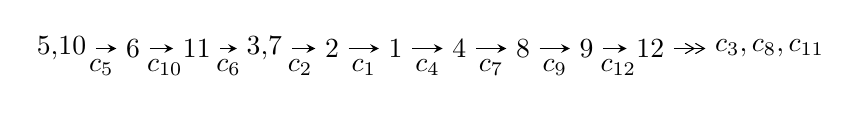
\begin{tikzpicture}[x=23pt, y=7pt]
	% node
	\node (A0) at (-1/8, 0) {5,10};
	\node (A1) at (1, 0) {6};
	\node (A2) at (2, 0) {11};
	\node (A3) at (49/16, 0) {3,7};
	\node (A4) at (33/8, 0) {2};
	\node (A5) at (41/8, 0) {1};
	\node (A6) at (49/8, 0) {4};
	\node (A7) at (57/8, 0) {8};
	\node (A8) at (65/8, 0) {9};
	\node (A9) at (73/8, 0) {12};
	\node (C1) at (1/2, -1) {$c_{5}$};
	\node (C2) at (3/2, -1) {$c_{10}$};
	\node (C3) at (5/2, -1) {$c_{6}$};
	\node (C4) at (29/8, -1) {$c_{2}$};
	\node (C5) at (37/8, -1) {$c_{1}$};
	\node (C6) at (45/8, -1) {$c_{4}$};
	\node (C7) at (53/8, -1) {$c_{7}$};
	\node (C8) at (61/8, -1) {$c_{9}$};
	\node (C9) at (69/8, -1) {$c_{12}$};
	\node (A10) at (11, 0) {$c_{3},c_{8},c_{11}$};

	% edge
	\draw[->,>=stealth]	
	(A0) edge (A1) (A1) edge (A2) (A2) edge (A3) (A3) edge (A4) (A4) edge (A5) (A5) edge (A6) (A6) edge (A7) (A7) edge (A8) (A8) edge (A9) ;
	\draw[->>,>={angle 60}]	
	(A9) edge (A10);
\end{tikzpicture} \\ 

\end{tabular} \\

\footnotetext{
The image of knot diagram is generated by the software ``\textbf{Draw programme}" developed by Andrew Bartholomew(\url{http://www.layer8.co.uk/maths/draw/index.htm\#Running-draw}), where we modified some parts for our purpose(\url{https://github.com/CATsTAILs/LinksPainter}).
}\phantom \\ \newline 
\centering \textbf{Ideals for irreducible components\footnotemark of $X_{\text{par}}$} 
 
\begin{align*}
I^u_{1}&=\langle 
-1.29904\times10^{129} u^{111}+2.66514\times10^{129} u^{110}+\cdots+3.21272\times10^{129} b+1.30058\times10^{129},\\
\phantom{I^u_{1}}&\phantom{= \langle  }5.52996\times10^{129} u^{111}-1.09032\times10^{130} u^{110}+\cdots+6.42545\times10^{129} a-1.03393\times10^{130},\\
\phantom{I^u_{1}}&\phantom{= \langle  }u^{112}-2 u^{111}+\cdots+24 u+8\rangle \\
I^u_{2}&=\langle 
b+1,\;2 u^7- u^6-5 u^5+2 u^4+3 u^3+a+2 u-1,\;u^8- u^7-3 u^6+2 u^5+3 u^4-2 u-1\rangle \\
I^u_{3}&=\langle 
32 a^2 u+14 a^2+6 a u+463 b+292 a+118 u-122,\;4 a^3+6 a^2 u-4 a^2+8 a u+3 u-20,\;u^2-2\rangle \\
\\
I^v_{1}&=\langle 
a,\;- v^2+b+3 v+1,\;v^3-2 v^2-3 v-1\rangle \\
\end{align*}
\raggedright * 4 irreducible components of $\dim_{\mathbb{C}}=0$, with total 129 representations.\\
\footnotetext{All coefficients of polynomials are rational numbers. But the coefficients are sometimes approximated in decimal forms when there is not enough margin.}
\newpage
\renewcommand{\arraystretch}{1}
\centering \section*{I. $I^u_{1}= \langle -1.30\times10^{129} u^{111}+2.67\times10^{129} u^{110}+\cdots+3.21\times10^{129} b+1.30\times10^{129},\;5.53\times10^{129} u^{111}-1.09\times10^{130} u^{110}+\cdots+6.43\times10^{129} a-1.03\times10^{130},\;u^{112}-2 u^{111}+\cdots+24 u+8 \rangle$}
\flushleft \textbf{(i) Arc colorings}\\
\begin{tabular}{m{7pt} m{180pt} m{7pt} m{180pt} }
\flushright $a_{5}=$&$\begin{pmatrix}1\\0\end{pmatrix}$ \\
\flushright $a_{10}=$&$\begin{pmatrix}0\\u\end{pmatrix}$ \\
\flushright $a_{6}=$&$\begin{pmatrix}1\\- u^2\end{pmatrix}$ \\
\flushright $a_{11}=$&$\begin{pmatrix}u\\- u^3+u\end{pmatrix}$ \\
\flushright $a_{3}=$&$\begin{pmatrix}-0.860634 u^{111}+1.69688 u^{110}+\cdots+1.28833 u+1.60912\\0.404343 u^{111}-0.829559 u^{110}+\cdots-2.02982 u-0.404820\end{pmatrix}$ \\
\flushright $a_{7}=$&$\begin{pmatrix}- u^2+1\\u^4-2 u^2\end{pmatrix}$ \\
\flushright $a_{2}=$&$\begin{pmatrix}-0.456291 u^{111}+0.867320 u^{110}+\cdots-0.741493 u+1.20430\\0.404343 u^{111}-0.829559 u^{110}+\cdots-2.02982 u-0.404820\end{pmatrix}$ \\
\flushright $a_{1}=$&$\begin{pmatrix}0.0400195 u^{111}-0.574902 u^{110}+\cdots+6.54098 u+2.08781\\-0.0638486 u^{111}+0.551541 u^{110}+\cdots-3.22913 u-1.01041\end{pmatrix}$ \\
\flushright $a_{4}=$&$\begin{pmatrix}0.278988 u^{111}-0.807051 u^{110}+\cdots+0.947750 u+3.03165\\-0.597516 u^{111}+1.47686 u^{110}+\cdots+0.793252 u-1.62436\end{pmatrix}$ \\
\flushright $a_{8}=$&$\begin{pmatrix}0.0413526 u^{111}-0.529064 u^{110}+\cdots+4.64588 u+1.51965\\0.183846 u^{111}+0.260857 u^{110}+\cdots-9.04776 u-3.12862\end{pmatrix}$ \\
\flushright $a_{9}=$&$\begin{pmatrix}- u^5+2 u^3- u\\u^7-3 u^5+2 u^3+u\end{pmatrix}$ \\
\flushright $a_{12}=$&$\begin{pmatrix}-0.0392866 u^{111}-0.413970 u^{110}+\cdots+9.42044 u+2.69703\\-0.101407 u^{111}+0.424993 u^{110}+\cdots-2.32534 u-0.770762\end{pmatrix}$\\&\end{tabular}
\flushleft \textbf{(ii) Obstruction class $= -1$}\\~\\
\flushleft \textbf{(iii) Cusp Shapes $= 1.31338 u^{111}-3.41480 u^{110}+\cdots+22.4635 u+1.55814$}\\~\\
\newpage\renewcommand{\arraystretch}{1}
\flushleft \textbf{(iv) u-Polynomials at the component}\newline \\
\begin{tabular}{m{50pt}|m{274pt}}
Crossings & \hspace{64pt}u-Polynomials at each crossing \\
\hline $$\begin{aligned}c_{1}\end{aligned}$$&$\begin{aligned}
&u^{112}+52 u^{111}+\cdots+2998 u+1
\end{aligned}$\\
\hline $$\begin{aligned}c_{2},c_{4}\end{aligned}$$&$\begin{aligned}
&u^{112}-12 u^{111}+\cdots+54 u+1
\end{aligned}$\\
\hline $$\begin{aligned}c_{3},c_{7}\end{aligned}$$&$\begin{aligned}
&u^{112}+2 u^{111}+\cdots+2688 u-256
\end{aligned}$\\
\hline $$\begin{aligned}c_{5},c_{6},c_{10}\end{aligned}$$&$\begin{aligned}
&u^{112}-2 u^{111}+\cdots+24 u+8
\end{aligned}$\\
\hline $$\begin{aligned}c_{8},c_{12}\end{aligned}$$&$\begin{aligned}
&u^{112}-5 u^{111}+\cdots-113 u+7
\end{aligned}$\\
\hline $$\begin{aligned}c_{9}\end{aligned}$$&$\begin{aligned}
&u^{112}+6 u^{111}+\cdots+84024 u+12200
\end{aligned}$\\
\hline $$\begin{aligned}c_{11}\end{aligned}$$&$\begin{aligned}
&u^{112}-57 u^{111}+\cdots-4733 u+49
\end{aligned}$\\
\hline
\end{tabular}\\~\\
\newpage\renewcommand{\arraystretch}{1}
\flushleft \textbf{(v) Riley Polynomials at the component}\newline \\
\begin{tabular}{m{50pt}|m{274pt}}
Crossings & \hspace{64pt}Riley Polynomials at each crossing \\
\hline $$\begin{aligned}c_{1}\end{aligned}$$&$\begin{aligned}
&y^{112}+28 y^{111}+\cdots-8620798 y+1
\end{aligned}$\\
\hline $$\begin{aligned}c_{2},c_{4}\end{aligned}$$&$\begin{aligned}
&y^{112}-52 y^{111}+\cdots-2998 y+1
\end{aligned}$\\
\hline $$\begin{aligned}c_{3},c_{7}\end{aligned}$$&$\begin{aligned}
&y^{112}+60 y^{111}+\cdots-3850240 y+65536
\end{aligned}$\\
\hline $$\begin{aligned}c_{5},c_{6},c_{10}\end{aligned}$$&$\begin{aligned}
&y^{112}-104 y^{111}+\cdots-960 y+64
\end{aligned}$\\
\hline $$\begin{aligned}c_{8},c_{12}\end{aligned}$$&$\begin{aligned}
&y^{112}-57 y^{111}+\cdots-4733 y+49
\end{aligned}$\\
\hline $$\begin{aligned}c_{9}\end{aligned}$$&$\begin{aligned}
&y^{112}-8 y^{111}+\cdots-4167168576 y+148840000
\end{aligned}$\\
\hline $$\begin{aligned}c_{11}\end{aligned}$$&$\begin{aligned}
&y^{112}+7 y^{111}+\cdots-16407805 y+2401
\end{aligned}$\\
\hline
\end{tabular}\\~\\
\newpage\flushleft \textbf{(vi) Complex Volumes and Cusp Shapes}
$$\begin{array}{c|c|c}  
\text{Solutions to }I^u_{1}& \I (\text{vol} + \sqrt{-1}CS) & \text{Cusp shape}\\
 \hline 
\begin{aligned}
u &= -1.018720 + 0.149036 I \\
a &= \phantom{-}0.076859 - 0.861231 I \\
b &= -1.158720 + 0.319869 I\end{aligned}
 & -1.29796 - 1.03206 I & \phantom{-0.000000 } 0 \\ \hline\begin{aligned}
u &= -1.018720 - 0.149036 I \\
a &= \phantom{-}0.076859 + 0.861231 I \\
b &= -1.158720 - 0.319869 I\end{aligned}
 & -1.29796 + 1.03206 I & \phantom{-0.000000 } 0 \\ \hline\begin{aligned}
u &= \phantom{-}0.814215 + 0.446584 I \\
a &= -0.037466 - 0.261223 I \\
b &= \phantom{-}1.067950 + 0.549015 I\end{aligned}
 & \phantom{-}0.00125 - 3.68506 I & \phantom{-0.000000 } 0 \\ \hline\begin{aligned}
u &= \phantom{-}0.814215 - 0.446584 I \\
a &= -0.037466 + 0.261223 I \\
b &= \phantom{-}1.067950 - 0.549015 I\end{aligned}
 & \phantom{-}0.00125 + 3.68506 I & \phantom{-0.000000 } 0 \\ \hline\begin{aligned}
u &= -0.711966 + 0.574552 I \\
a &= -0.174449 + 0.367324 I \\
b &= \phantom{-}1.131830 - 0.614451 I\end{aligned}
 & \phantom{-}1.90412 + 8.94633 I & \phantom{-0.000000 } 0 \\ \hline\begin{aligned}
u &= -0.711966 - 0.574552 I \\
a &= -0.174449 - 0.367324 I \\
b &= \phantom{-}1.131830 + 0.614451 I\end{aligned}
 & \phantom{-}1.90412 - 8.94633 I & \phantom{-0.000000 } 0 \\ \hline\begin{aligned}
u &= \phantom{-}1.036270 + 0.398425 I \\
a &= \phantom{-}0.447897 + 0.876758 I \\
b &= \phantom{-}0.979382 - 0.404050 I\end{aligned}
 & -0.78854 + 2.81223 I & \phantom{-0.000000 } 0 \\ \hline\begin{aligned}
u &= \phantom{-}1.036270 - 0.398425 I \\
a &= \phantom{-}0.447897 - 0.876758 I \\
b &= \phantom{-}0.979382 + 0.404050 I\end{aligned}
 & -0.78854 - 2.81223 I & \phantom{-0.000000 } 0 \\ \hline\begin{aligned}
u &= \phantom{-}1.116570 + 0.051427 I \\
a &= \phantom{-}0.657850 - 0.997380 I \\
b &= -0.177665 + 0.553771 I\end{aligned}
 & \phantom{-}1.74796 + 0.16171 I & \phantom{-0.000000 } 0 \\ \hline\begin{aligned}
u &= \phantom{-}1.116570 - 0.051427 I \\
a &= \phantom{-}0.657850 + 0.997380 I \\
b &= -0.177665 - 0.553771 I\end{aligned}
 & \phantom{-}1.74796 - 0.16171 I & \phantom{-0.000000 } 0\\
 \hline 
 \end{array}$$\newpage$$\begin{array}{c|c|c}  
\text{Solutions to }I^u_{1}& \I (\text{vol} + \sqrt{-1}CS) & \text{Cusp shape}\\
 \hline 
\begin{aligned}
u &= \phantom{-}1.110930 + 0.219371 I \\
a &= -0.14481 - 1.71768 I \\
b &= -1.153040 + 0.367430 I\end{aligned}
 & -1.22070 + 3.54389 I & \phantom{-0.000000 } 0 \\ \hline\begin{aligned}
u &= \phantom{-}1.110930 - 0.219371 I \\
a &= -0.14481 + 1.71768 I \\
b &= -1.153040 - 0.367430 I\end{aligned}
 & -1.22070 - 3.54389 I & \phantom{-0.000000 } 0 \\ \hline\begin{aligned}
u &= -0.355833 + 0.788222 I \\
a &= \phantom{-}1.05625 - 1.50575 I \\
b &= \phantom{-}1.170610 + 0.637818 I\end{aligned}
 & \phantom{-}0.72546 - 13.62000 I & \phantom{-0.000000 -}0. + 9.98825 I \\ \hline\begin{aligned}
u &= -0.355833 - 0.788222 I \\
a &= \phantom{-}1.05625 + 1.50575 I \\
b &= \phantom{-}1.170610 - 0.637818 I\end{aligned}
 & \phantom{-}0.72546 + 13.62000 I & \phantom{-0.000000 } 0. - 9.98825 I \\ \hline\begin{aligned}
u &= \phantom{-}0.146754 + 0.822078 I \\
a &= \phantom{-}0.893745 + 0.277347 I \\
b &= \phantom{-}0.911228 + 0.313596 I\end{aligned}
 & -3.54227 + 1.59081 I & \phantom{-}1.56582 + 2.52489 I \\ \hline\begin{aligned}
u &= \phantom{-}0.146754 - 0.822078 I \\
a &= \phantom{-}0.893745 - 0.277347 I \\
b &= \phantom{-}0.911228 - 0.313596 I\end{aligned}
 & -3.54227 - 1.59081 I & \phantom{-}1.56582 - 2.52489 I \\ \hline\begin{aligned}
u &= -1.167790 + 0.097848 I \\
a &= \phantom{-}0.725202 - 0.286646 I \\
b &= \phantom{-}0.881268 - 0.521081 I\end{aligned}
 & \phantom{-}6.34503 + 2.09810 I & \phantom{-0.000000 } 0 \\ \hline\begin{aligned}
u &= -1.167790 - 0.097848 I \\
a &= \phantom{-}0.725202 + 0.286646 I \\
b &= \phantom{-}0.881268 + 0.521081 I\end{aligned}
 & \phantom{-}6.34503 - 2.09810 I & \phantom{-0.000000 } 0 \\ \hline\begin{aligned}
u &= -0.624872 + 0.541441 I \\
a &= \phantom{-}0.485440 - 1.097800 I \\
b &= \phantom{-}0.392106 + 0.829105 I\end{aligned}
 & \phantom{-}4.11190 + 3.56494 I & \phantom{-}7.21254 - 1.29951 I \\ \hline\begin{aligned}
u &= -0.624872 - 0.541441 I \\
a &= \phantom{-}0.485440 + 1.097800 I \\
b &= \phantom{-}0.392106 - 0.829105 I\end{aligned}
 & \phantom{-}4.11190 - 3.56494 I & \phantom{-}7.21254 + 1.29951 I\\
 \hline 
 \end{array}$$\newpage$$\begin{array}{c|c|c}  
\text{Solutions to }I^u_{1}& \I (\text{vol} + \sqrt{-1}CS) & \text{Cusp shape}\\
 \hline 
\begin{aligned}
u &= \phantom{-}0.274658 + 0.777797 I \\
a &= \phantom{-}1.28184 + 1.22191 I \\
b &= \phantom{-}1.134650 - 0.590961 I\end{aligned}
 & -1.75122 + 8.04540 I & -0.69722 - 6.48181 I \\ \hline\begin{aligned}
u &= \phantom{-}0.274658 - 0.777797 I \\
a &= \phantom{-}1.28184 - 1.22191 I \\
b &= \phantom{-}1.134650 + 0.590961 I\end{aligned}
 & -1.75122 - 8.04540 I & -0.69722 + 6.48181 I \\ \hline\begin{aligned}
u &= -0.011399 + 0.820861 I \\
a &= \phantom{-}1.141370 + 0.028393 I \\
b &= \phantom{-}1.003200 - 0.397478 I\end{aligned}
 & -4.15841 + 4.21135 I & -1.12819 - 7.26950 I \\ \hline\begin{aligned}
u &= -0.011399 - 0.820861 I \\
a &= \phantom{-}1.141370 - 0.028393 I \\
b &= \phantom{-}1.003200 + 0.397478 I\end{aligned}
 & -4.15841 - 4.21135 I & -1.12819 + 7.26950 I \\ \hline\begin{aligned}
u &= -0.358023 + 0.736800 I \\
a &= -0.605113 + 0.240449 I \\
b &= \phantom{-}0.369589 - 0.924331 I\end{aligned}
 & \phantom{-}3.15487 - 7.91029 I & \phantom{-}5.30872 + 6.56414 I \\ \hline\begin{aligned}
u &= -0.358023 - 0.736800 I \\
a &= -0.605113 - 0.240449 I \\
b &= \phantom{-}0.369589 + 0.924331 I\end{aligned}
 & \phantom{-}3.15487 + 7.91029 I & \phantom{-}5.30872 - 6.56414 I \\ \hline\begin{aligned}
u &= \phantom{-}0.303360 + 0.725677 I \\
a &= -0.65527 - 1.79904 I \\
b &= -1.015110 + 0.566452 I\end{aligned}
 & -1.69797 + 7.17522 I & \phantom{-}0.68379 - 7.57915 I \\ \hline\begin{aligned}
u &= \phantom{-}0.303360 - 0.725677 I \\
a &= -0.65527 + 1.79904 I \\
b &= -1.015110 - 0.566452 I\end{aligned}
 & -1.69797 - 7.17522 I & \phantom{-}0.68379 + 7.57915 I \\ \hline\begin{aligned}
u &= \phantom{-}0.652565 + 0.422024 I \\
a &= \phantom{-}0.774209 + 0.886160 I \\
b &= -0.995831 - 0.466362 I\end{aligned}
 & -0.38831 - 3.14093 I & \phantom{-}2.48859 + 2.59563 I \\ \hline\begin{aligned}
u &= \phantom{-}0.652565 - 0.422024 I \\
a &= \phantom{-}0.774209 - 0.886160 I \\
b &= -0.995831 + 0.466362 I\end{aligned}
 & -0.38831 + 3.14093 I & \phantom{-}2.48859 - 2.59563 I\\
 \hline 
 \end{array}$$\newpage$$\begin{array}{c|c|c}  
\text{Solutions to }I^u_{1}& \I (\text{vol} + \sqrt{-1}CS) & \text{Cusp shape}\\
 \hline 
\begin{aligned}
u &= -1.217770 + 0.231362 I \\
a &= \phantom{-}0.066728 + 0.949450 I \\
b &= \phantom{-}0.002019 - 0.679432 I\end{aligned}
 & \phantom{-}2.29898 - 4.70132 I & \phantom{-0.000000 } 0 \\ \hline\begin{aligned}
u &= -1.217770 - 0.231362 I \\
a &= \phantom{-}0.066728 - 0.949450 I \\
b &= \phantom{-}0.002019 + 0.679432 I\end{aligned}
 & \phantom{-}2.29898 + 4.70132 I & \phantom{-0.000000 } 0 \\ \hline\begin{aligned}
u &= -0.263923 + 0.703760 I \\
a &= -0.978990 + 0.422628 I \\
b &= -1.309070 + 0.166176 I\end{aligned}
 & -2.65149 - 4.51648 I & \phantom{-}1.07409 + 6.59561 I \\ \hline\begin{aligned}
u &= -0.263923 - 0.703760 I \\
a &= -0.978990 - 0.422628 I \\
b &= -1.309070 - 0.166176 I\end{aligned}
 & -2.65149 + 4.51648 I & \phantom{-}1.07409 - 6.59561 I \\ \hline\begin{aligned}
u &= \phantom{-}0.294109 + 0.686488 I \\
a &= -0.364849 + 0.009699 I \\
b &= \phantom{-}0.339982 + 0.789548 I\end{aligned}
 & \phantom{-}0.57903 + 2.86162 I & \phantom{-}2.21640 - 3.05288 I \\ \hline\begin{aligned}
u &= \phantom{-}0.294109 - 0.686488 I \\
a &= -0.364849 - 0.009699 I \\
b &= \phantom{-}0.339982 - 0.789548 I\end{aligned}
 & \phantom{-}0.57903 - 2.86162 I & \phantom{-}2.21640 + 3.05288 I \\ \hline\begin{aligned}
u &= -1.196320 + 0.379749 I \\
a &= \phantom{-}0.446586 - 1.195840 I \\
b &= \phantom{-}1.071020 + 0.461092 I\end{aligned}
 & -0.50009 - 8.52415 I & \phantom{-0.000000 } 0 \\ \hline\begin{aligned}
u &= -1.196320 - 0.379749 I \\
a &= \phantom{-}0.446586 + 1.195840 I \\
b &= \phantom{-}1.071020 - 0.461092 I\end{aligned}
 & -0.50009 + 8.52415 I & \phantom{-0.000000 } 0 \\ \hline\begin{aligned}
u &= \phantom{-}0.584146 + 0.424260 I \\
a &= \phantom{-}0.495792 + 0.880233 I \\
b &= \phantom{-}0.508203 - 0.602695 I\end{aligned}
 & \phantom{-}1.72036 + 0.90594 I & \phantom{-}4.78781 - 4.00969 I \\ \hline\begin{aligned}
u &= \phantom{-}0.584146 - 0.424260 I \\
a &= \phantom{-}0.495792 - 0.880233 I \\
b &= \phantom{-}0.508203 + 0.602695 I\end{aligned}
 & \phantom{-}1.72036 - 0.90594 I & \phantom{-}4.78781 + 4.00969 I\\
 \hline 
 \end{array}$$\newpage$$\begin{array}{c|c|c}  
\text{Solutions to }I^u_{1}& \I (\text{vol} + \sqrt{-1}CS) & \text{Cusp shape}\\
 \hline 
\begin{aligned}
u &= \phantom{-}1.229960 + 0.360736 I \\
a &= \phantom{-}0.037108 + 0.251367 I \\
b &= \phantom{-}0.915433 + 0.334717 I\end{aligned}
 & -0.329456 + 0.040199 I & \phantom{-0.000000 } 0 \\ \hline\begin{aligned}
u &= \phantom{-}1.229960 - 0.360736 I \\
a &= \phantom{-}0.037108 - 0.251367 I \\
b &= \phantom{-}0.915433 - 0.334717 I\end{aligned}
 & -0.329456 - 0.040199 I & \phantom{-0.000000 } 0 \\ \hline\begin{aligned}
u &= -0.654491 + 0.272544 I \\
a &= \phantom{-}0.04579 + 1.78125 I \\
b &= -1.182700 - 0.184351 I\end{aligned}
 & -1.085270 + 0.846553 I & \phantom{-}3.79032 - 3.13132 I \\ \hline\begin{aligned}
u &= -0.654491 - 0.272544 I \\
a &= \phantom{-}0.04579 - 1.78125 I \\
b &= -1.182700 + 0.184351 I\end{aligned}
 & -1.085270 - 0.846553 I & \phantom{-}3.79032 + 3.13132 I \\ \hline\begin{aligned}
u &= -0.188194 + 0.675147 I \\
a &= -1.11851 + 1.65238 I \\
b &= -1.051720 - 0.452819 I\end{aligned}
 & -3.69167 - 2.26136 I & -3.60384 + 2.58351 I \\ \hline\begin{aligned}
u &= -0.188194 - 0.675147 I \\
a &= -1.11851 - 1.65238 I \\
b &= -1.051720 + 0.452819 I\end{aligned}
 & -3.69167 + 2.26136 I & -3.60384 - 2.58351 I \\ \hline\begin{aligned}
u &= \phantom{-}0.240940 + 0.637061 I \\
a &= \phantom{-}0.719669 + 0.632063 I \\
b &= -0.562579 - 0.604506 I\end{aligned}
 & -0.34785 + 2.50804 I & \phantom{-}1.82220 - 3.40193 I \\ \hline\begin{aligned}
u &= \phantom{-}0.240940 - 0.637061 I \\
a &= \phantom{-}0.719669 - 0.632063 I \\
b &= -0.562579 + 0.604506 I\end{aligned}
 & -0.34785 - 2.50804 I & \phantom{-}1.82220 + 3.40193 I \\ \hline\begin{aligned}
u &= \phantom{-}0.112061 + 0.664682 I \\
a &= -1.48275 + 0.14053 I \\
b &= -1.214020 - 0.246890 I\end{aligned}
 & -4.20929 - 0.20936 I & -3.46102 - 1.21494 I \\ \hline\begin{aligned}
u &= \phantom{-}0.112061 - 0.664682 I \\
a &= -1.48275 - 0.14053 I \\
b &= -1.214020 + 0.246890 I\end{aligned}
 & -4.20929 + 0.20936 I & -3.46102 + 1.21494 I\\
 \hline 
 \end{array}$$\newpage$$\begin{array}{c|c|c}  
\text{Solutions to }I^u_{1}& \I (\text{vol} + \sqrt{-1}CS) & \text{Cusp shape}\\
 \hline 
\begin{aligned}
u &= -1.327970 + 0.003111 I \\
a &= -0.87431 + 1.66645 I \\
b &= \phantom{-}0.894917 - 0.825816 I\end{aligned}
 & \phantom{-}8.09882 + 3.06301 I & \phantom{-0.000000 } 0 \\ \hline\begin{aligned}
u &= -1.327970 - 0.003111 I \\
a &= -0.87431 - 1.66645 I \\
b &= \phantom{-}0.894917 + 0.825816 I\end{aligned}
 & \phantom{-}8.09882 - 3.06301 I & \phantom{-0.000000 } 0 \\ \hline\begin{aligned}
u &= \phantom{-}1.324830 + 0.184519 I \\
a &= \phantom{-}1.29142 + 1.08887 I \\
b &= -0.530536 - 0.575105 I\end{aligned}
 & \phantom{-}2.68371 + 1.14617 I & \phantom{-0.000000 } 0 \\ \hline\begin{aligned}
u &= \phantom{-}1.324830 - 0.184519 I \\
a &= \phantom{-}1.29142 - 1.08887 I \\
b &= -0.530536 + 0.575105 I\end{aligned}
 & \phantom{-}2.68371 - 1.14617 I & \phantom{-0.000000 } 0 \\ \hline\begin{aligned}
u &= -0.332085 + 0.570168 I \\
a &= -0.823871 - 0.740483 I \\
b &= \phantom{-}0.570546 - 0.745691 I\end{aligned}
 & \phantom{-}5.19659 + 0.52268 I & \phantom{-}7.07371 + 1.25938 I \\ \hline\begin{aligned}
u &= -0.332085 - 0.570168 I \\
a &= -0.823871 + 0.740483 I \\
b &= \phantom{-}0.570546 + 0.745691 I\end{aligned}
 & \phantom{-}5.19659 - 0.52268 I & \phantom{-}7.07371 - 1.25938 I \\ \hline\begin{aligned}
u &= -0.213775 + 0.619265 I \\
a &= \phantom{-}2.33602 - 1.25730 I \\
b &= \phantom{-}1.026980 + 0.623990 I\end{aligned}
 & \phantom{-}3.82789 - 4.68728 I & \phantom{-}3.46609 + 6.29400 I \\ \hline\begin{aligned}
u &= -0.213775 - 0.619265 I \\
a &= \phantom{-}2.33602 + 1.25730 I \\
b &= \phantom{-}1.026980 - 0.623990 I\end{aligned}
 & \phantom{-}3.82789 + 4.68728 I & \phantom{-}3.46609 - 6.29400 I \\ \hline\begin{aligned}
u &= -1.339170 + 0.244598 I \\
a &= \phantom{-}0.128580 + 0.409997 I \\
b &= -1.292610 + 0.172501 I\end{aligned}
 & \phantom{-}0.35822 - 3.05224 I & \phantom{-0.000000 } 0 \\ \hline\begin{aligned}
u &= -1.339170 - 0.244598 I \\
a &= \phantom{-}0.128580 - 0.409997 I \\
b &= -1.292610 - 0.172501 I\end{aligned}
 & \phantom{-}0.35822 + 3.05224 I & \phantom{-0.000000 } 0\\
 \hline 
 \end{array}$$\newpage$$\begin{array}{c|c|c}  
\text{Solutions to }I^u_{1}& \I (\text{vol} + \sqrt{-1}CS) & \text{Cusp shape}\\
 \hline 
\begin{aligned}
u &= -0.003632 + 0.612874 I \\
a &= \phantom{-}0.533006 - 0.318247 I \\
b &= -0.213424 + 0.523869 I\end{aligned}
 & -1.41839 + 1.56464 I & -0.45093 - 4.40997 I \\ \hline\begin{aligned}
u &= -0.003632 - 0.612874 I \\
a &= \phantom{-}0.533006 + 0.318247 I \\
b &= -0.213424 - 0.523869 I\end{aligned}
 & -1.41839 - 1.56464 I & -0.45093 + 4.40997 I \\ \hline\begin{aligned}
u &= -1.38959\phantom{ +0.000000I} \\
a &= \phantom{-}0.908732\phantom{ +0.000000I} \\
b &= -0.0184563\phantom{ +0.000000I}\end{aligned}
 & \phantom{-}6.53354\phantom{ +0.000000I} & \phantom{-0.000000 } 0 \\ \hline\begin{aligned}
u &= -1.346640 + 0.354641 I \\
a &= -0.027424 - 0.336567 I \\
b &= \phantom{-}0.849993 - 0.240388 I\end{aligned}
 & \phantom{-}1.14529 - 5.82695 I & \phantom{-0.000000 } 0 \\ \hline\begin{aligned}
u &= -1.346640 - 0.354641 I \\
a &= -0.027424 + 0.336567 I \\
b &= \phantom{-}0.849993 + 0.240388 I\end{aligned}
 & \phantom{-}1.14529 + 5.82695 I & \phantom{-0.000000 } 0 \\ \hline\begin{aligned}
u &= \phantom{-}1.372090 + 0.263367 I \\
a &= \phantom{-}0.10678 - 2.41007 I \\
b &= -1.015250 + 0.548202 I\end{aligned}
 & \phantom{-}1.26200 + 5.66357 I & \phantom{-0.000000 } 0 \\ \hline\begin{aligned}
u &= \phantom{-}1.372090 - 0.263367 I \\
a &= \phantom{-}0.10678 + 2.41007 I \\
b &= -1.015250 - 0.548202 I\end{aligned}
 & \phantom{-}1.26200 - 5.66357 I & \phantom{-0.000000 } 0 \\ \hline\begin{aligned}
u &= \phantom{-}1.389480 + 0.176832 I \\
a &= -1.12892 - 1.39935 I \\
b &= \phantom{-}1.035730 + 0.807448 I\end{aligned}
 & \phantom{-}9.96290 + 0.00502 I & \phantom{-0.000000 } 0 \\ \hline\begin{aligned}
u &= \phantom{-}1.389480 - 0.176832 I \\
a &= -1.12892 + 1.39935 I \\
b &= \phantom{-}1.035730 - 0.807448 I\end{aligned}
 & \phantom{-}9.96290 - 0.00502 I & \phantom{-0.000000 } 0 \\ \hline\begin{aligned}
u &= -0.333286 + 0.497276 I \\
a &= \phantom{-}0.205344 - 0.950156 I \\
b &= \phantom{-}0.722048 + 0.843897 I\end{aligned}
 & \phantom{-}5.42986 - 3.71507 I & \phantom{-}6.56090 + 8.40821 I\\
 \hline 
 \end{array}$$\newpage$$\begin{array}{c|c|c}  
\text{Solutions to }I^u_{1}& \I (\text{vol} + \sqrt{-1}CS) & \text{Cusp shape}\\
 \hline 
\begin{aligned}
u &= -0.333286 - 0.497276 I \\
a &= \phantom{-}0.205344 + 0.950156 I \\
b &= \phantom{-}0.722048 - 0.843897 I\end{aligned}
 & \phantom{-}5.42986 + 3.71507 I & \phantom{-}6.56090 - 8.40821 I \\ \hline\begin{aligned}
u &= \phantom{-}1.398300 + 0.107009 I \\
a &= -0.59433 - 1.65394 I \\
b &= -1.165440 - 0.052793 I\end{aligned}
 & \phantom{-}5.03887 + 0.33340 I & \phantom{-0.000000 } 0 \\ \hline\begin{aligned}
u &= \phantom{-}1.398300 - 0.107009 I \\
a &= -0.59433 + 1.65394 I \\
b &= -1.165440 + 0.052793 I\end{aligned}
 & \phantom{-}5.03887 - 0.33340 I & \phantom{-0.000000 } 0 \\ \hline\begin{aligned}
u &= -1.394040 + 0.168090 I \\
a &= -0.05486 + 2.88093 I \\
b &= -0.899734 - 0.466308 I\end{aligned}
 & \phantom{-}6.09712 - 2.33253 I & \phantom{-0.000000 } 0 \\ \hline\begin{aligned}
u &= -1.394040 - 0.168090 I \\
a &= -0.05486 - 2.88093 I \\
b &= -0.899734 + 0.466308 I\end{aligned}
 & \phantom{-}6.09712 + 2.33253 I & \phantom{-0.000000 } 0 \\ \hline\begin{aligned}
u &= \phantom{-}1.386180 + 0.248074 I \\
a &= \phantom{-}0.67456 + 2.27430 I \\
b &= \phantom{-}1.098480 - 0.642310 I\end{aligned}
 & \phantom{-}8.93573 + 7.87318 I & \phantom{-0.000000 } 0 \\ \hline\begin{aligned}
u &= \phantom{-}1.386180 - 0.248074 I \\
a &= \phantom{-}0.67456 - 2.27430 I \\
b &= \phantom{-}1.098480 + 0.642310 I\end{aligned}
 & \phantom{-}8.93573 - 7.87318 I & \phantom{-0.000000 } 0 \\ \hline\begin{aligned}
u &= -1.39563 + 0.25220 I \\
a &= \phantom{-}1.35096 - 1.26835 I \\
b &= -0.652912 + 0.690244 I\end{aligned}
 & \phantom{-}4.87673 - 5.76508 I & \phantom{-0.000000 } 0 \\ \hline\begin{aligned}
u &= -1.39563 - 0.25220 I \\
a &= \phantom{-}1.35096 + 1.26835 I \\
b &= -0.652912 - 0.690244 I\end{aligned}
 & \phantom{-}4.87673 + 5.76508 I & \phantom{-0.000000 } 0 \\ \hline\begin{aligned}
u &= \phantom{-}1.41403 + 0.20520 I \\
a &= -0.39049 + 1.93565 I \\
b &= \phantom{-}0.695558 - 0.941026 I\end{aligned}
 & \phantom{-}10.99240 + 6.37614 I & \phantom{-0.000000 } 0\\
 \hline 
 \end{array}$$\newpage$$\begin{array}{c|c|c}  
\text{Solutions to }I^u_{1}& \I (\text{vol} + \sqrt{-1}CS) & \text{Cusp shape}\\
 \hline 
\begin{aligned}
u &= \phantom{-}1.41403 - 0.20520 I \\
a &= -0.39049 - 1.93565 I \\
b &= \phantom{-}0.695558 + 0.941026 I\end{aligned}
 & \phantom{-}10.99240 - 6.37614 I & \phantom{-0.000000 } 0 \\ \hline\begin{aligned}
u &= \phantom{-}1.43186\phantom{ +0.000000I} \\
a &= \phantom{-}7.47358\phantom{ +0.000000I} \\
b &= -0.970695\phantom{ +0.000000I}\end{aligned}
 & \phantom{-}4.97680\phantom{ +0.000000I} & \phantom{-0.000000 } 0 \\ \hline\begin{aligned}
u &= \phantom{-}1.40615 + 0.27781 I \\
a &= \phantom{-}0.451286 - 0.581959 I \\
b &= -1.358830 - 0.131787 I\end{aligned}
 & \phantom{-}2.67390 + 8.08693 I & \phantom{-0.000000 } 0 \\ \hline\begin{aligned}
u &= \phantom{-}1.40615 - 0.27781 I \\
a &= \phantom{-}0.451286 + 0.581959 I \\
b &= -1.358830 + 0.131787 I\end{aligned}
 & \phantom{-}2.67390 - 8.08693 I & \phantom{-0.000000 } 0 \\ \hline\begin{aligned}
u &= \phantom{-}1.42100 + 0.21744 I \\
a &= -1.228290 - 0.553828 I \\
b &= \phantom{-}0.474203 + 0.831698 I\end{aligned}
 & \phantom{-}10.80900 + 2.37680 I & \phantom{-0.000000 } 0 \\ \hline\begin{aligned}
u &= \phantom{-}1.42100 - 0.21744 I \\
a &= -1.228290 + 0.553828 I \\
b &= \phantom{-}0.474203 - 0.831698 I\end{aligned}
 & \phantom{-}10.80900 - 2.37680 I & \phantom{-0.000000 } 0 \\ \hline\begin{aligned}
u &= -1.41572 + 0.27049 I \\
a &= -0.978454 + 0.922450 I \\
b &= \phantom{-}0.368700 - 0.903629 I\end{aligned}
 & \phantom{-}6.03543 - 6.35471 I & \phantom{-0.000000 } 0 \\ \hline\begin{aligned}
u &= -1.41572 - 0.27049 I \\
a &= -0.978454 - 0.922450 I \\
b &= \phantom{-}0.368700 + 0.903629 I\end{aligned}
 & \phantom{-}6.03543 + 6.35471 I & \phantom{-0.000000 } 0 \\ \hline\begin{aligned}
u &= -1.44321 + 0.10269 I \\
a &= -0.43536 - 1.61858 I \\
b &= \phantom{-}0.716567 + 0.769054 I\end{aligned}
 & \phantom{-}8.22583 - 2.63796 I & \phantom{-0.000000 } 0 \\ \hline\begin{aligned}
u &= -1.44321 - 0.10269 I \\
a &= -0.43536 + 1.61858 I \\
b &= \phantom{-}0.716567 - 0.769054 I\end{aligned}
 & \phantom{-}8.22583 + 2.63796 I & \phantom{-0.000000 } 0\\
 \hline 
 \end{array}$$\newpage$$\begin{array}{c|c|c}  
\text{Solutions to }I^u_{1}& \I (\text{vol} + \sqrt{-1}CS) & \text{Cusp shape}\\
 \hline 
\begin{aligned}
u &= -1.41705 + 0.31061 I \\
a &= \phantom{-}0.23451 - 2.12729 I \\
b &= \phantom{-}1.162710 + 0.631820 I\end{aligned}
 & \phantom{-}3.63940 - 11.98600 I & \phantom{-0.000000 } 0 \\ \hline\begin{aligned}
u &= -1.41705 - 0.31061 I \\
a &= \phantom{-}0.23451 + 2.12729 I \\
b &= \phantom{-}1.162710 - 0.631820 I\end{aligned}
 & \phantom{-}3.63940 + 11.98600 I & \phantom{-0.000000 } 0 \\ \hline\begin{aligned}
u &= -1.42523 + 0.28547 I \\
a &= \phantom{-}0.28388 + 2.43754 I \\
b &= -0.995964 - 0.623300 I\end{aligned}
 & \phantom{-}3.82611 - 10.85450 I & \phantom{-0.000000 } 0 \\ \hline\begin{aligned}
u &= -1.42523 - 0.28547 I \\
a &= \phantom{-}0.28388 - 2.43754 I \\
b &= -0.995964 + 0.623300 I\end{aligned}
 & \phantom{-}3.82611 + 10.85450 I & \phantom{-0.000000 } 0 \\ \hline\begin{aligned}
u &= -1.46859 + 0.11194 I \\
a &= \phantom{-}1.69922 - 1.26036 I \\
b &= -0.841564 + 0.435407 I\end{aligned}
 & \phantom{-}6.34093 + 1.39160 I & \phantom{-0.000000 } 0 \\ \hline\begin{aligned}
u &= -1.46859 - 0.11194 I \\
a &= \phantom{-}1.69922 + 1.26036 I \\
b &= -0.841564 - 0.435407 I\end{aligned}
 & \phantom{-}6.34093 - 1.39160 I & \phantom{-0.000000 } 0 \\ \hline\begin{aligned}
u &= \phantom{-}1.45063 + 0.28488 I \\
a &= -1.11139 - 1.11493 I \\
b &= \phantom{-}0.397230 + 0.978223 I\end{aligned}
 & \phantom{-}8.9567 + 11.6332 I & \phantom{-0.000000 } 0 \\ \hline\begin{aligned}
u &= \phantom{-}1.45063 - 0.28488 I \\
a &= -1.11139 + 1.11493 I \\
b &= \phantom{-}0.397230 - 0.978223 I\end{aligned}
 & \phantom{-}8.9567 - 11.6332 I & \phantom{-0.000000 } 0 \\ \hline\begin{aligned}
u &= \phantom{-}1.45761 + 0.30717 I \\
a &= \phantom{-}0.05506 + 2.27142 I \\
b &= \phantom{-}1.184370 - 0.665894 I\end{aligned}
 & \phantom{-}6.5408 + 17.6016 I & \phantom{-0.000000 } 0 \\ \hline\begin{aligned}
u &= \phantom{-}1.45761 - 0.30717 I \\
a &= \phantom{-}0.05506 - 2.27142 I \\
b &= \phantom{-}1.184370 + 0.665894 I\end{aligned}
 & \phantom{-}6.5408 - 17.6016 I & \phantom{-0.000000 } 0\\
 \hline 
 \end{array}$$\newpage$$\begin{array}{c|c|c}  
\text{Solutions to }I^u_{1}& \I (\text{vol} + \sqrt{-1}CS) & \text{Cusp shape}\\
 \hline 
\begin{aligned}
u &= -1.50703 + 0.02402 I \\
a &= -0.74209 + 1.21258 I \\
b &= \phantom{-}0.927314 - 0.617513 I\end{aligned}
 & \phantom{-}7.63433 + 2.61707 I & \phantom{-0.000000 } 0 \\ \hline\begin{aligned}
u &= -1.50703 - 0.02402 I \\
a &= -0.74209 - 1.21258 I \\
b &= \phantom{-}0.927314 + 0.617513 I\end{aligned}
 & \phantom{-}7.63433 - 2.61707 I & \phantom{-0.000000 } 0 \\ \hline\begin{aligned}
u &= \phantom{-}1.50704 + 0.14911 I \\
a &= -0.10240 + 1.73413 I \\
b &= \phantom{-}0.513892 - 0.813284 I\end{aligned}
 & \phantom{-}11.06290 - 1.16602 I & \phantom{-0.000000 } 0 \\ \hline\begin{aligned}
u &= \phantom{-}1.50704 - 0.14911 I \\
a &= -0.10240 - 1.73413 I \\
b &= \phantom{-}0.513892 + 0.813284 I\end{aligned}
 & \phantom{-}11.06290 + 1.16602 I & \phantom{-0.000000 } 0 \\ \hline\begin{aligned}
u &= -0.237025 + 0.395062 I \\
a &= \phantom{-}0.003829 + 0.713299 I \\
b &= \phantom{-}0.958789 - 0.771571 I\end{aligned}
 & \phantom{-}4.74030 + 2.24272 I & \phantom{-}3.61623 + 6.16785 I \\ \hline\begin{aligned}
u &= -0.237025 - 0.395062 I \\
a &= \phantom{-}0.003829 - 0.713299 I \\
b &= \phantom{-}0.958789 + 0.771571 I\end{aligned}
 & \phantom{-}4.74030 - 2.24272 I & \phantom{-}3.61623 - 6.16785 I \\ \hline\begin{aligned}
u &= \phantom{-}1.53699 + 0.12427 I \\
a &= -0.99596 - 1.13045 I \\
b &= \phantom{-}1.073900 + 0.645562 I\end{aligned}
 & \phantom{-}9.38113 - 6.62724 I & \phantom{-0.000000 } 0 \\ \hline\begin{aligned}
u &= \phantom{-}1.53699 - 0.12427 I \\
a &= -0.99596 + 1.13045 I \\
b &= \phantom{-}1.073900 - 0.645562 I\end{aligned}
 & \phantom{-}9.38113 + 6.62724 I & \phantom{-0.000000 } 0 \\ \hline\begin{aligned}
u &= \phantom{-}0.276680 + 0.321195 I \\
a &= -0.57913 - 4.82110 I \\
b &= -0.757806 + 0.273988 I\end{aligned}
 & \phantom{-}0.771024 + 0.267712 I & \phantom{-}2.70998 - 9.56080 I \\ \hline\begin{aligned}
u &= \phantom{-}0.276680 - 0.321195 I \\
a &= -0.57913 + 4.82110 I \\
b &= -0.757806 - 0.273988 I\end{aligned}
 & \phantom{-}0.771024 - 0.267712 I & \phantom{-}2.70998 + 9.56080 I\\
 \hline 
 \end{array}$$\newpage$$\begin{array}{c|c|c}  
\text{Solutions to }I^u_{1}& \I (\text{vol} + \sqrt{-1}CS) & \text{Cusp shape}\\
 \hline 
\begin{aligned}
u &= \phantom{-}0.417834\phantom{ +0.000000I} \\
a &= \phantom{-}1.69611\phantom{ +0.000000I} \\
b &= -0.141393\phantom{ +0.000000I}\end{aligned}
 & \phantom{-}0.992954\phantom{ +0.000000I} & \phantom{-}11.5370\phantom{ +0.000000I} \\ \hline\begin{aligned}
u &= -0.236458\phantom{ +0.000000I} \\
a &= \phantom{-}2.76698\phantom{ +0.000000I} \\
b &= -0.881202\phantom{ +0.000000I}\end{aligned}
 & -1.26916\phantom{ +0.000000I} & -9.80040\phantom{ +0.000000I}\\
 \hline 
 \end{array}$$\newpage\newpage\renewcommand{\arraystretch}{1}
\centering \section*{II. $I^u_{2}= \langle b+1,\;2 u^7- u^6-5 u^5+2 u^4+3 u^3+a+2 u-1,\;u^8- u^7-3 u^6+2 u^5+3 u^4-2 u-1 \rangle$}
\flushleft \textbf{(i) Arc colorings}\\
\begin{tabular}{m{7pt} m{180pt} m{7pt} m{180pt} }
\flushright $a_{5}=$&$\begin{pmatrix}1\\0\end{pmatrix}$ \\
\flushright $a_{10}=$&$\begin{pmatrix}0\\u\end{pmatrix}$ \\
\flushright $a_{6}=$&$\begin{pmatrix}1\\- u^2\end{pmatrix}$ \\
\flushright $a_{11}=$&$\begin{pmatrix}u\\- u^3+u\end{pmatrix}$ \\
\flushright $a_{3}=$&$\begin{pmatrix}-2 u^7+u^6+5 u^5-2 u^4-3 u^3-2 u+1\\-1\end{pmatrix}$ \\
\flushright $a_{7}=$&$\begin{pmatrix}- u^2+1\\u^4-2 u^2\end{pmatrix}$ \\
\flushright $a_{2}=$&$\begin{pmatrix}-2 u^7+u^6+5 u^5-2 u^4-3 u^3-2 u\\-1\end{pmatrix}$ \\
\flushright $a_{1}=$&$\begin{pmatrix}-1\\0\end{pmatrix}$ \\
\flushright $a_{4}=$&$\begin{pmatrix}-2 u^7+u^6+5 u^5-2 u^4-3 u^3-2 u+1\\-1\end{pmatrix}$ \\
\flushright $a_{8}=$&$\begin{pmatrix}- u^2+1\\u^4-2 u^2\end{pmatrix}$ \\
\flushright $a_{9}=$&$\begin{pmatrix}- u^5+2 u^3- u\\u^7-3 u^5+2 u^3+u\end{pmatrix}$ \\
\flushright $a_{12}=$&$\begin{pmatrix}- u^3+2 u\\- u^3+u\end{pmatrix}$\\&\end{tabular}
\flushleft \textbf{(ii) Obstruction class $= 1$}\\~\\
\flushleft \textbf{(iii) Cusp Shapes $= 4 u^7+9 u^6-10 u^5-27 u^4-2 u^3+18 u^2+20 u+17$}\\~\\
\newpage\renewcommand{\arraystretch}{1}
\flushleft \textbf{(iv) u-Polynomials at the component}\newline \\
\begin{tabular}{m{50pt}|m{274pt}}
Crossings & \hspace{64pt}u-Polynomials at each crossing \\
\hline $$\begin{aligned}c_{1},c_{2}\end{aligned}$$&$\begin{aligned}
&(u-1)^8
\end{aligned}$\\
\hline $$\begin{aligned}c_{3},c_{7}\end{aligned}$$&$\begin{aligned}
&u^8
\end{aligned}$\\
\hline $$\begin{aligned}c_{4}\end{aligned}$$&$\begin{aligned}
&(u+1)^8
\end{aligned}$\\
\hline $$\begin{aligned}c_{5},c_{6}\end{aligned}$$&$\begin{aligned}
&u^8- u^7-3 u^6+2 u^5+3 u^4-2 u-1
\end{aligned}$\\
\hline $$\begin{aligned}c_{8}\end{aligned}$$&$\begin{aligned}
&u^8+u^7- u^6-2 u^5+u^4+2 u^3-2 u-1
\end{aligned}$\\
\hline $$\begin{aligned}c_{9}\end{aligned}$$&$\begin{aligned}
&u^8-3 u^7+7 u^6-10 u^5+11 u^4-10 u^3+6 u^2-4 u+1
\end{aligned}$\\
\hline $$\begin{aligned}c_{10}\end{aligned}$$&$\begin{aligned}
&u^8+u^7-3 u^6-2 u^5+3 u^4+2 u-1
\end{aligned}$\\
\hline $$\begin{aligned}c_{11}\end{aligned}$$&$\begin{aligned}
&u^8+3 u^7+7 u^6+10 u^5+11 u^4+10 u^3+6 u^2+4 u+1
\end{aligned}$\\
\hline $$\begin{aligned}c_{12}\end{aligned}$$&$\begin{aligned}
&u^8- u^7- u^6+2 u^5+u^4-2 u^3+2 u-1
\end{aligned}$\\
\hline
\end{tabular}\\~\\
\newpage\renewcommand{\arraystretch}{1}
\flushleft \textbf{(v) Riley Polynomials at the component}\newline \\
\begin{tabular}{m{50pt}|m{274pt}}
Crossings & \hspace{64pt}Riley Polynomials at each crossing \\
\hline $$\begin{aligned}c_{1},c_{2},c_{4}\end{aligned}$$&$\begin{aligned}
&(y-1)^8
\end{aligned}$\\
\hline $$\begin{aligned}c_{3},c_{7}\end{aligned}$$&$\begin{aligned}
&y^8
\end{aligned}$\\
\hline $$\begin{aligned}c_{5},c_{6},c_{10}\end{aligned}$$&$\begin{aligned}
&y^8-7 y^7+19 y^6-22 y^5+3 y^4+14 y^3-6 y^2-4 y+1
\end{aligned}$\\
\hline $$\begin{aligned}c_{8},c_{12}\end{aligned}$$&$\begin{aligned}
&y^8-3 y^7+7 y^6-10 y^5+11 y^4-10 y^3+6 y^2-4 y+1
\end{aligned}$\\
\hline $$\begin{aligned}c_{9},c_{11}\end{aligned}$$&$\begin{aligned}
&y^8+5 y^7+11 y^6+6 y^5-17 y^4-34 y^3-22 y^2-4 y+1
\end{aligned}$\\
\hline
\end{tabular}\\~\\
\newpage\flushleft \textbf{(vi) Complex Volumes and Cusp Shapes}
$$\begin{array}{c|c|c}  
\text{Solutions to }I^u_{2}& \I (\text{vol} + \sqrt{-1}CS) & \text{Cusp shape}\\
 \hline 
\begin{aligned}
u &= -1.180120 + 0.268597 I \\
a &= -0.085690 + 0.514779 I \\
b &= -1.00000\phantom{ +0.000000I}\end{aligned}
 & -0.604279 - 1.131230 I & \phantom{-}1.38132 + 1.25921 I \\ \hline\begin{aligned}
u &= -1.180120 - 0.268597 I \\
a &= -0.085690 - 0.514779 I \\
b &= -1.00000\phantom{ +0.000000I}\end{aligned}
 & -0.604279 + 1.131230 I & \phantom{-}1.38132 - 1.25921 I \\ \hline\begin{aligned}
u &= -0.108090 + 0.747508 I \\
a &= -1.036110 + 0.260696 I \\
b &= -1.00000\phantom{ +0.000000I}\end{aligned}
 & -3.80435 - 2.57849 I & -1.74277 + 4.63100 I \\ \hline\begin{aligned}
u &= -0.108090 - 0.747508 I \\
a &= -1.036110 - 0.260696 I \\
b &= -1.00000\phantom{ +0.000000I}\end{aligned}
 & -3.80435 + 2.57849 I & -1.74277 - 4.63100 I \\ \hline\begin{aligned}
u &= \phantom{-}1.37100\phantom{ +0.000000I} \\
a &= -3.88842\phantom{ +0.000000I} \\
b &= -1.00000\phantom{ +0.000000I}\end{aligned}
 & \phantom{-}4.85780\phantom{ +0.000000I} & \phantom{-}25.4550\phantom{ +0.000000I} \\ \hline\begin{aligned}
u &= \phantom{-}1.334530 + 0.318930 I \\
a &= \phantom{-}0.043072 - 0.634428 I \\
b &= -1.00000\phantom{ +0.000000I}\end{aligned}
 & \phantom{-}0.73474 + 6.44354 I & \phantom{-}1.71699 - 7.87618 I \\ \hline\begin{aligned}
u &= \phantom{-}1.334530 - 0.318930 I \\
a &= \phantom{-}0.043072 + 0.634428 I \\
b &= -1.00000\phantom{ +0.000000I}\end{aligned}
 & \phantom{-}0.73474 - 6.44354 I & \phantom{-}1.71699 + 7.87618 I \\ \hline\begin{aligned}
u &= -0.463640\phantom{ +0.000000I} \\
a &= \phantom{-}2.04588\phantom{ +0.000000I} \\
b &= -1.00000\phantom{ +0.000000I}\end{aligned}
 & -0.799899\phantom{ +0.000000I} & \phantom{-}10.8330\phantom{ +0.000000I}\\
 \hline 
 \end{array}$$\newpage\newpage\renewcommand{\arraystretch}{1}
\centering \section*{III. $I^u_{3}= \langle 32 a^2 u+6 a u+\cdots+292 a-122,\;4 a^3+6 a^2 u-4 a^2+8 a u+3 u-20,\;u^2-2 \rangle$}
\flushleft \textbf{(i) Arc colorings}\\
\begin{tabular}{m{7pt} m{180pt} m{7pt} m{180pt} }
\flushright $a_{5}=$&$\begin{pmatrix}1\\0\end{pmatrix}$ \\
\flushright $a_{10}=$&$\begin{pmatrix}0\\u\end{pmatrix}$ \\
\flushright $a_{6}=$&$\begin{pmatrix}1\\-2\end{pmatrix}$ \\
\flushright $a_{11}=$&$\begin{pmatrix}u\\- u\end{pmatrix}$ \\
\flushright $a_{3}=$&$\begin{pmatrix}a\\-0.0691145 a^{2} u-0.0129590 a u+\cdots-0.630670 a+0.263499\end{pmatrix}$ \\
\flushright $a_{7}=$&$\begin{pmatrix}-1\\0\end{pmatrix}$ \\
\flushright $a_{2}=$&$\begin{pmatrix}-0.0691145 a^{2} u-0.0129590 a u+\cdots+0.369330 a+0.263499\\-0.0691145 a^{2} u-0.0129590 a u+\cdots-0.630670 a+0.263499\end{pmatrix}$ \\
\flushright $a_{1}=$&$\begin{pmatrix}0.0604752 a^{2} u+0.261339 a u+\cdots+0.0518359 a-0.980562\\-0.0604752 a^{2} u-0.261339 a u+\cdots-0.0518359 a+0.980562\end{pmatrix}$ \\
\flushright $a_{4}=$&$\begin{pmatrix}0.0453564 a^{2} u-0.0539957 a u+\cdots+0.0388769 a+0.764579\\0.00863931 a^{2} u-0.248380 a u+\cdots+0.578834 a-0.282937\end{pmatrix}$ \\
\flushright $a_{8}=$&$\begin{pmatrix}0.0604752 a^{2} u+0.261339 a u+\cdots+0.0518359 a-0.980562\\-0.0604752 a^{2} u-0.261339 a u+\cdots-0.0518359 a+0.980562\end{pmatrix}$ \\
\flushright $a_{9}=$&$\begin{pmatrix}- u\\u\end{pmatrix}$ \\
\flushright $a_{12}=$&$\begin{pmatrix}0.0604752 a^{2} u+0.261339 a u+\cdots+0.0518359 a-0.980562\\-0.0604752 a^{2} u-0.261339 a u+\cdots-0.0518359 a+0.980562\end{pmatrix}$\\&\end{tabular}
\flushleft \textbf{(ii) Obstruction class $= 1$}\\~\\
\flushleft \textbf{(iii) Cusp Shapes $= -\frac{128}{463} a^2 u-\frac{56}{463} a^2-\frac{24}{463} a u-\frac{1168}{463} a-\frac{472}{463} u+\frac{4192}{463}$}\\~\\
\newpage\renewcommand{\arraystretch}{1}
\flushleft \textbf{(iv) u-Polynomials at the component}\newline \\
\begin{tabular}{m{50pt}|m{274pt}}
Crossings & \hspace{64pt}u-Polynomials at each crossing \\
\hline $$\begin{aligned}c_{1},c_{7}\end{aligned}$$&$\begin{aligned}
&(u^3- u^2+2 u-1)^2
\end{aligned}$\\
\hline $$\begin{aligned}c_{2}\end{aligned}$$&$\begin{aligned}
&(u^3+u^2-1)^2
\end{aligned}$\\
\hline $$\begin{aligned}c_{3}\end{aligned}$$&$\begin{aligned}
&(u^3+u^2+2 u+1)^2
\end{aligned}$\\
\hline $$\begin{aligned}c_{4}\end{aligned}$$&$\begin{aligned}
&(u^3- u^2+1)^2
\end{aligned}$\\
\hline $$\begin{aligned}c_{5},c_{6},c_{9}\\c_{10}\end{aligned}$$&$\begin{aligned}
&(u^2-2)^3
\end{aligned}$\\
\hline $$\begin{aligned}c_{8}\end{aligned}$$&$\begin{aligned}
&(u-1)^6
\end{aligned}$\\
\hline $$\begin{aligned}c_{11},c_{12}\end{aligned}$$&$\begin{aligned}
&(u+1)^6
\end{aligned}$\\
\hline
\end{tabular}\\~\\
\newpage\renewcommand{\arraystretch}{1}
\flushleft \textbf{(v) Riley Polynomials at the component}\newline \\
\begin{tabular}{m{50pt}|m{274pt}}
Crossings & \hspace{64pt}Riley Polynomials at each crossing \\
\hline $$\begin{aligned}c_{1},c_{3},c_{7}\end{aligned}$$&$\begin{aligned}
&(y^3+3 y^2+2 y-1)^2
\end{aligned}$\\
\hline $$\begin{aligned}c_{2},c_{4}\end{aligned}$$&$\begin{aligned}
&(y^3- y^2+2 y-1)^2
\end{aligned}$\\
\hline $$\begin{aligned}c_{5},c_{6},c_{9}\\c_{10}\end{aligned}$$&$\begin{aligned}
&(y-2)^6
\end{aligned}$\\
\hline $$\begin{aligned}c_{8},c_{11},c_{12}\end{aligned}$$&$\begin{aligned}
&(y-1)^6
\end{aligned}$\\
\hline
\end{tabular}\\~\\
\newpage\flushleft \textbf{(vi) Complex Volumes and Cusp Shapes}
$$\begin{array}{c|c|c}  
\text{Solutions to }I^u_{3}& \I (\text{vol} + \sqrt{-1}CS) & \text{Cusp shape}\\
 \hline 
\begin{aligned}
u &= \phantom{-}1.41421\phantom{ +0.000000I} \\
a &= \phantom{-}0.865932\phantom{ +0.000000I} \\
b &= -0.754878\phantom{ +0.000000I}\end{aligned}
 & \phantom{-}5.46628\phantom{ +0.000000I} & \phantom{-}4.98050\phantom{ +0.000000I} \\ \hline\begin{aligned}
u &= \phantom{-}1.41421\phantom{ +0.000000I} \\
a &= -0.99363 + 1.88732 I \\
b &= \phantom{-}0.877439 - 0.744862 I\end{aligned}
 & \phantom{-}9.60386 + 2.82812 I & \phantom{-}11.50976 - 2.97945 I \\ \hline\begin{aligned}
u &= \phantom{-}1.41421\phantom{ +0.000000I} \\
a &= -0.99363 - 1.88732 I \\
b &= \phantom{-}0.877439 + 0.744862 I\end{aligned}
 & \phantom{-}9.60386 - 2.82812 I & \phantom{-}11.50976 + 2.97945 I \\ \hline\begin{aligned}
u &= -1.41421\phantom{ +0.000000I} \\
a &= -0.516129 + 1.092130 I \\
b &= \phantom{-}0.877439 - 0.744862 I\end{aligned}
 & \phantom{-}9.60386 + 2.82812 I & \phantom{-}11.50976 - 2.97945 I \\ \hline\begin{aligned}
u &= -1.41421\phantom{ +0.000000I} \\
a &= -0.516129 - 1.092130 I \\
b &= \phantom{-}0.877439 + 0.744862 I\end{aligned}
 & \phantom{-}9.60386 - 2.82812 I & \phantom{-}11.50976 + 2.97945 I \\ \hline\begin{aligned}
u &= -1.41421\phantom{ +0.000000I} \\
a &= \phantom{-}4.15358\phantom{ +0.000000I} \\
b &= -0.754878\phantom{ +0.000000I}\end{aligned}
 & \phantom{-}5.46628\phantom{ +0.000000I} & \phantom{-}4.98050\phantom{ +0.000000I}\\
 \hline 
 \end{array}$$\newpage\newpage\renewcommand{\arraystretch}{1}
\centering \section*{IV. $I^v_{1}= \langle a,\;- v^2+b+3 v+1,\;v^3-2 v^2-3 v-1 \rangle$}
\flushleft \textbf{(i) Arc colorings}\\
\begin{tabular}{m{7pt} m{180pt} m{7pt} m{180pt} }
\flushright $a_{5}=$&$\begin{pmatrix}1\\0\end{pmatrix}$ \\
\flushright $a_{10}=$&$\begin{pmatrix}v\\0\end{pmatrix}$ \\
\flushright $a_{6}=$&$\begin{pmatrix}1\\0\end{pmatrix}$ \\
\flushright $a_{11}=$&$\begin{pmatrix}v\\0\end{pmatrix}$ \\
\flushright $a_{3}=$&$\begin{pmatrix}0\\v^2-3 v-1\end{pmatrix}$ \\
\flushright $a_{7}=$&$\begin{pmatrix}1\\0\end{pmatrix}$ \\
\flushright $a_{2}=$&$\begin{pmatrix}v^2-3 v-1\\v^2-3 v-1\end{pmatrix}$ \\
\flushright $a_{1}=$&$\begin{pmatrix}v^2-3 v-1\\- v^2+2 v+3\end{pmatrix}$ \\
\flushright $a_{4}=$&$\begin{pmatrix}-2 v^2+5 v+4\\-2 v^2+5 v+3\end{pmatrix}$ \\
\flushright $a_{8}=$&$\begin{pmatrix}- v^2+3 v+1\\v^2-2 v-3\end{pmatrix}$ \\
\flushright $a_{9}=$&$\begin{pmatrix}v\\0\end{pmatrix}$ \\
\flushright $a_{12}=$&$\begin{pmatrix}v^2-2 v-1\\- v^2+2 v+3\end{pmatrix}$\\&\end{tabular}
\flushleft \textbf{(ii) Obstruction class $= 1$}\\~\\
\flushleft \textbf{(iii) Cusp Shapes $= 8 v^2-26 v-14$}\\~\\
\newpage\renewcommand{\arraystretch}{1}
\flushleft \textbf{(iv) u-Polynomials at the component}\newline \\
\begin{tabular}{m{50pt}|m{274pt}}
Crossings & \hspace{64pt}u-Polynomials at each crossing \\
\hline $$\begin{aligned}c_{1},c_{3}\end{aligned}$$&$\begin{aligned}
&u^3- u^2+2 u-1
\end{aligned}$\\
\hline $$\begin{aligned}c_{2}\end{aligned}$$&$\begin{aligned}
&u^3+u^2-1
\end{aligned}$\\
\hline $$\begin{aligned}c_{4}\end{aligned}$$&$\begin{aligned}
&u^3- u^2+1
\end{aligned}$\\
\hline $$\begin{aligned}c_{5},c_{6},c_{9}\\c_{10}\end{aligned}$$&$\begin{aligned}
&u^3
\end{aligned}$\\
\hline $$\begin{aligned}c_{7}\end{aligned}$$&$\begin{aligned}
&u^3+u^2+2 u+1
\end{aligned}$\\
\hline $$\begin{aligned}c_{8},c_{11}\end{aligned}$$&$\begin{aligned}
&(u+1)^3
\end{aligned}$\\
\hline $$\begin{aligned}c_{12}\end{aligned}$$&$\begin{aligned}
&(u-1)^3
\end{aligned}$\\
\hline
\end{tabular}\\~\\
\newpage\renewcommand{\arraystretch}{1}
\flushleft \textbf{(v) Riley Polynomials at the component}\newline \\
\begin{tabular}{m{50pt}|m{274pt}}
Crossings & \hspace{64pt}Riley Polynomials at each crossing \\
\hline $$\begin{aligned}c_{1},c_{3},c_{7}\end{aligned}$$&$\begin{aligned}
&y^3+3 y^2+2 y-1
\end{aligned}$\\
\hline $$\begin{aligned}c_{2},c_{4}\end{aligned}$$&$\begin{aligned}
&y^3- y^2+2 y-1
\end{aligned}$\\
\hline $$\begin{aligned}c_{5},c_{6},c_{9}\\c_{10}\end{aligned}$$&$\begin{aligned}
&y^3
\end{aligned}$\\
\hline $$\begin{aligned}c_{8},c_{11},c_{12}\end{aligned}$$&$\begin{aligned}
&(y-1)^3
\end{aligned}$\\
\hline
\end{tabular}\\~\\
\newpage\flushleft \textbf{(vi) Complex Volumes and Cusp Shapes}
$$\begin{array}{c|c|c}  
\text{Solutions to }I^v_{1}& \I (\text{vol} + \sqrt{-1}CS) & \text{Cusp shape}\\
 \hline 
\begin{aligned}
v &= -0.539798 + 0.182582 I \\
a &= \phantom{-0.000000 } 0 \\
b &= \phantom{-}0.877439 - 0.744862 I\end{aligned}
 & \phantom{-}4.66906 + 2.82812 I & \phantom{-}2.09911 - 6.32406 I \\ \hline\begin{aligned}
v &= -0.539798 - 0.182582 I \\
a &= \phantom{-0.000000 } 0 \\
b &= \phantom{-}0.877439 + 0.744862 I\end{aligned}
 & \phantom{-}4.66906 - 2.82812 I & \phantom{-}2.09911 + 6.32406 I \\ \hline\begin{aligned}
v &= \phantom{-}3.07960\phantom{ +0.000000I} \\
a &= \phantom{-0.000000 } 0 \\
b &= -0.754878\phantom{ +0.000000I}\end{aligned}
 & \phantom{-}0.531480\phantom{ +0.000000I} & -18.1980\phantom{ +0.000000I}\\
 \hline 
 \end{array}$$\newpage
\newpage\renewcommand{\arraystretch}{1}
\centering \section*{ V. u-Polynomials}
\begin{tabular}{m{50pt}|m{274pt}}
Crossings & \hspace{64pt}u-Polynomials at each crossing \\
\hline $$\begin{aligned}c_{1}\end{aligned}$$&$\begin{aligned}
&((u-1)^8)(u^3- u^2+2 u-1)^3(u^{112}+52 u^{111}+\cdots+2998 u+1)
\end{aligned}$\\
\hline $$\begin{aligned}c_{2}\end{aligned}$$&$\begin{aligned}
&((u-1)^8)(u^3+u^2-1)^3(u^{112}-12 u^{111}+\cdots+54 u+1)
\end{aligned}$\\
\hline $$\begin{aligned}c_{3}\end{aligned}$$&$\begin{aligned}
&u^8(u^3- u^2+2 u-1)(u^3+u^2+2 u+1)^2\\
&\cdot(u^{112}+2 u^{111}+\cdots+2688 u-256)
\end{aligned}$\\
\hline $$\begin{aligned}c_{4}\end{aligned}$$&$\begin{aligned}
&((u+1)^8)(u^3- u^2+1)^3(u^{112}-12 u^{111}+\cdots+54 u+1)
\end{aligned}$\\
\hline $$\begin{aligned}c_{5},c_{6}\end{aligned}$$&$\begin{aligned}
&u^3(u^2-2)^3(u^8- u^7-3 u^6+2 u^5+3 u^4-2 u-1)\\
&\cdot(u^{112}-2 u^{111}+\cdots+24 u+8)
\end{aligned}$\\
\hline $$\begin{aligned}c_{7}\end{aligned}$$&$\begin{aligned}
&u^8(u^3- u^2+2 u-1)^2(u^3+u^2+2 u+1)\\
&\cdot(u^{112}+2 u^{111}+\cdots+2688 u-256)
\end{aligned}$\\
\hline $$\begin{aligned}c_{8}\end{aligned}$$&$\begin{aligned}
&(u-1)^6(u+1)^3(u^8+u^7- u^6-2 u^5+u^4+2 u^3-2 u-1)\\
&\cdot(u^{112}-5 u^{111}+\cdots-113 u+7)
\end{aligned}$\\
\hline $$\begin{aligned}c_{9}\end{aligned}$$&$\begin{aligned}
&u^3(u^2-2)^3(u^8-3 u^7+7 u^6-10 u^5+11 u^4-10 u^3+6 u^2-4 u+1)\\
&\cdot(u^{112}+6 u^{111}+\cdots+84024 u+12200)
\end{aligned}$\\
\hline $$\begin{aligned}c_{10}\end{aligned}$$&$\begin{aligned}
&u^3(u^2-2)^3(u^8+u^7-3 u^6-2 u^5+3 u^4+2 u-1)\\
&\cdot(u^{112}-2 u^{111}+\cdots+24 u+8)
\end{aligned}$\\
\hline $$\begin{aligned}c_{11}\end{aligned}$$&$\begin{aligned}
&(u+1)^9(u^8+3 u^7+7 u^6+10 u^5+11 u^4+10 u^3+6 u^2+4 u+1)\\
&\cdot(u^{112}-57 u^{111}+\cdots-4733 u+49)
\end{aligned}$\\
\hline $$\begin{aligned}c_{12}\end{aligned}$$&$\begin{aligned}
&(u-1)^3(u+1)^6(u^8- u^7- u^6+2 u^5+u^4-2 u^3+2 u-1)\\
&\cdot(u^{112}-5 u^{111}+\cdots-113 u+7)
\end{aligned}$\\
\hline
\end{tabular}\newpage\renewcommand{\arraystretch}{1}
\centering \section*{ VI. Riley Polynomials}
\begin{tabular}{m{50pt}|m{274pt}}
Crossings & \hspace{64pt}Riley Polynomials at each crossing \\
\hline $$\begin{aligned}c_{1}\end{aligned}$$&$\begin{aligned}
&((y-1)^8)(y^3+3 y^2+2 y-1)^3(y^{112}+28 y^{111}+\cdots-8620798 y+1)
\end{aligned}$\\
\hline $$\begin{aligned}c_{2},c_{4}\end{aligned}$$&$\begin{aligned}
&((y-1)^8)(y^3- y^2+2 y-1)^3(y^{112}-52 y^{111}+\cdots-2998 y+1)
\end{aligned}$\\
\hline $$\begin{aligned}c_{3},c_{7}\end{aligned}$$&$\begin{aligned}
&y^8(y^3+3 y^2+2 y-1)^3(y^{112}+60 y^{111}+\cdots-3850240 y+65536)
\end{aligned}$\\
\hline $$\begin{aligned}c_{5},c_{6},c_{10}\end{aligned}$$&$\begin{aligned}
&y^3(y-2)^6(y^8-7 y^7+19 y^6-22 y^5+3 y^4+14 y^3-6 y^2-4 y+1)\\
&\cdot(y^{112}-104 y^{111}+\cdots-960 y+64)
\end{aligned}$\\
\hline $$\begin{aligned}c_{8},c_{12}\end{aligned}$$&$\begin{aligned}
&(y-1)^9(y^8-3 y^7+7 y^6-10 y^5+11 y^4-10 y^3+6 y^2-4 y+1)\\
&\cdot(y^{112}-57 y^{111}+\cdots-4733 y+49)
\end{aligned}$\\
\hline $$\begin{aligned}c_{9}\end{aligned}$$&$\begin{aligned}
&y^3(y-2)^6(y^8+5 y^7+11 y^6+6 y^5-17 y^4-34 y^3-22 y^2-4 y+1)\\
&\cdot(y^{112}-8 y^{111}+\cdots-4167168576 y+148840000)
\end{aligned}$\\
\hline $$\begin{aligned}c_{11}\end{aligned}$$&$\begin{aligned}
&(y-1)^9(y^8+5 y^7+11 y^6+6 y^5-17 y^4-34 y^3-22 y^2-4 y+1)\\
&\cdot(y^{112}+7 y^{111}+\cdots-16407805 y+2401)
\end{aligned}$\\
\hline
\end{tabular}
\vskip 2pc
\end{document}